\documentclass{article}
\usepackage[T1]{fontenc} % add special characters (e.g., umlaute)
\usepackage[utf8]{inputenc} % set utf-8 as default input encoding
\usepackage{ismir,amsmath,cite,url}
\usepackage{graphicx}
\usepackage{color}


\usepackage{comment}
\usepackage{verbatim}
\usepackage{moreverb}
\usepackage{multirow}

\usepackage{algorithm}
\usepackage[noend]{algpseudocode}
\usepackage{minted}

\usepackage{pgfplots}
\usepgfplotslibrary{statistics}
\usepackage{tikz}


\newtheorem{Definition}{Definition}
\newtheorem{Example}{Example}

\newtheorem{Theorem}{Theorem}
\newtheorem{Proposition}[Theorem]{Proposition}
\newtheorem{Remark}{Remark}

\graphicspath{{../score-examples/}}

\def\neuma/{\textsc{NEUMA}}
\def\munir/{\textsc{MuNIR}}
\def\alphabet/{\ensuremath{{\cal E}}}
\def\exact/{\textsc{Ex}}
\def\ryth/{\textsc{Ry}}
\def\transp/{\textsc{Tr}}
\def\exhaus/{\textsc{Sc}}
\def\elasticsearch/{\textsc{ElasticSearch}}

\newcommand{\vect}[1]{\ensuremath{\textbf{\rm{#1}}}}

 \def\durations/{\ensuremath{{\cal D}}}
\newcommand{\fig}[2]
{
\begin{figure}[ht]
 \centerline{
 \includegraphics[width=\columnwidth]{#1}}
	\vspace*{-.3cm}
 \caption{\label{#1} #2}
\end{figure}
} 

\newcommand{\figWithSize}[3]
{
\begin{figure}[ht]
 \centerline{
 \includegraphics[width=#3]{#1}}
	\vspace*{-.3cm}
 \caption{\label{#1} #2}
\end{figure}
}

\newcommand{\FigWithSize}[3]
{
	\begin{figure*}[ht]
		\centerline{
			\includegraphics[width=#3]{#1}}
		\caption{\label{#1} #2}
	\end{figure*}
}

\newenvironment{longue}{}{}%
\newenvironment{courte}{\textbf{}}{}

\newenvironment{smallverbatim}%
{\endgraf\small\verbatimtab}{\endverbatimtab}


\newcommand{\promille}{%
  \relax\ifmmode\promillezeichen
        \else\leavevmode\(\mathsurround=0pt\promillezeichen\)\fi}
\newcommand{\promillezeichen}{%
  \kern-.05em%
  \raise.5ex\hbox{\the\scriptfont0 0}%
  \kern-.15em/\kern-.15em%
  \lower.25ex\hbox{\the\scriptfont0 00}}
  
  

\definecolor{mygray}{gray}{0.90}
\definecolor{mygreen}{rgb}{0,0.5,0}
\definecolor{maroon}{rgb}{0.5,0,0}
\newcommand{\remPR}[1]{%
\vspace*{0.1cm}
\hrule
\medskip
\noindent
\textbf{\textcolor{maroon}{Philippe}}: \textit{#1}
\medskip
\hrule
\vspace*{0.1cm}
}


\newcommand{\remNT}[1]{%
\vspace*{0.1cm}
\hrule
\medskip
\noindent
\textbf{\textcolor{mygreen}{Nicolas}}: \textit{#1}
\medskip
\hrule
\vspace*{0.1cm}
}


\title{Scalable Searching and Ranking\\  for Melodic Pattern Queries}


\twoauthors
{Philippe Rigaux} {Cedric Lab, CNAM\\ {\tt philippe.rigaux@cnam.fr}}
{Nicolas Travers} {Leonard de Vinci, Research Center\\Cedric Lab, CNAM\\ {\tt nicolas.travers@devinci.fr}}

%\threeauthors
%{First Author} {Affiliation1 \\ {\tt author1@ismir.edu}}
%{Second Author} {\bf Retain these fake authors in\\\bf submission to preserve the formatting}
%{Third Author} {Affiliation3 \\ {\tt author3@ismir.edu}}

\sloppy

\begin{document}

%
\maketitle

%
\begin{abstract}
We present the design and implementation of a scalable search engine for large Digital Score 
Libraries. It covers the core features expected from an information retrieval system. 
Music representation is pre-processed, simplified and normalized.
Collections are searched for scores that match
a melodic pattern, results are ranked on their similarity with the pattern, and matching fragments 
are finally identified on the fly. 
Moreover, all these features are designed to be integrated in a standard
search engine and thus benefit from the horizontal scalability
of such systems. Our method is fully implemented, and relies
on \elasticsearch/ for collection indexing. We describe its main components,
report and study its performances.
%All the components are released in open source on Github for the community of people and institutions managing large collections of digitized scores.
\end{abstract}

\section{Introduction}\label{sec:intro}

We consider the problem of searching large collections of digital scores
encoded in a symbolic format, 
typically MusicXML~\cite{Good01},  MEI~\cite{Rolland02,MEI_ws},
or the forthcoming format of the W3C Music Notation Group~\cite{MNX_overview}. These encodings are now mature
and stable, and we can expect to witness in the near future the emergence
of very large Digital Score Libraries (DSL). A representative example of such endeavors is
the OpenScore initiative, %(\url{http://openscore.cc}),
 which aims at publishing high-quality encoding of
public domain sheet music. This potentially represents millions of scores, and
gives rise to strong needs in terms of collection management tools tailored to the
peculiarities of music representation.

In the present paper, we focus on the \emph{content-based retrieval} problem. 
We consider the search mechanism where a user submits
a monophonic \emph{query pattern} in order to retrieve, from a very large
collection of scores, those that contain one or more fragments ``similar'' to this pattern. 
We further require the search system to be \emph{scalable}.
% dealing with instant response time.
%Our assumptions on scores, fragments, and patterns, as well as scalability requirements, are developped in the first section of the paper.

With this objective in mind, we propose two main contributions.
First, we expose the design of the core modules of a search engine, namely 
pre-processing and data normalization, pattern-based search, ranking, 
and on-line identification of fragments that match the  pattern query.  
Second, we propose a list of guidelines for integrating these modules in a standard information retrieval
system, with two main benefits: reduction of implementation efforts, and horizontal scalability.

\begin{figure*}[ht]
	\centerline{
		\includegraphics[width=\linewidth]{../figures/matching-steps2}}
	\vspace*{-.35cm}
	\caption{\label{../figures/matching-steps} Overview of the main indexing and matching steps}
\end{figure*}

Our approach is summarized by Figure~\ref{../figures/matching-steps}. Pre-proces\-sing, matching,
occurrence extraction and ranking are standard steps in text-based information retrieval systems, adapted 
here to
the specificities of music representation. Tokenization, stemming and lemmatization~\cite{MRS08} 
are, in our case, replaced by a so-called \emph{normalization}
that simplifies the representation and improves the robustness of the result. 
The \emph{matching step} operates on the normalized representation (query pattern and score content). Normalization
and matching are detailed in Section~\ref{sec:search}.

Obtaining a full score in the result %of a pattern-based query 
would be of little
use if we were not able to identify all the fragments that actually match the pattern,
called \emph{pattern occurrences}. This is necessary,  for instance,
to highlight them in the user interface.
%Occurrences identification operates on the full score representation. 
The  algorithm is
described in  Section~\ref{sec:highlight}.

Finally, the set of matching scores  are sorted according to 
the similarity of their occurrences to the pattern. While pattern matching mostly relies 
on the melodic profile, the ranking
method focuses on the rhythm (Section~\ref{sec:rank}). Their combination produces results  with highly relevant scores. %regarding both criteria are top-ranked.
%The ranking method is presented in .

The rest of the paper (Section~\ref{sec:implem}) covers our second contribution, namely the integration
of our music retrieval components  in a standard search engine. For the sake of concreteness, we
detail this integration with \elasticsearch/ (\url{https://elastic.co}).%, however the method is actually applicable to any system relying on standard inverted index structures. 
%We also give a brief description of our DSL, \neuma/, featuring
%a search interface that benefits from these search functions.

We finally  position our work with respect to the state of the art
and lists some useful extensions that could enrich the search functionalities (Section~\ref{sec:rw}).

%\smallskip

%The paper is deliberately  practice-oriented. Anyone wishing to equip a score library with a search  mechanism should be able to do so quite easily by following our methodology.
%To this end, we also created  a GitHub repository  where our components are freely available.

%%%%%%%%%%%%%%5
\section{Preliminaries: scores, fragments, and patterns}\label{sec:prelim} 

Given a \emph{melodic pattern} $P$ as input, the \emph{pattern matching operation}
retrieves all the \emph{scores} such that at least one \emph{fragment} matches $P$.
%
%The concepts
%of scores, fragments, patterns and matching are defined in turn, and illustrated by the example 
%of Figure~\ref{incipit-44} that shows the initial measures of a typical music score.   
%
%\fig{incipit-44}{Excerpt of a polyphonic score}
%
%Although it would be
%possible, in principle, to build a search system addressing all the components of this layout
%(beams, slurs, annotations, directions)
Our approach focuses on the pitch and duration features,
generally considered as the most important parameters for melodic similarity~\cite{Prince14}.  We model 
a score as a synchronization of \emph{voices}, and each voice as a sequence of  elements $<e_1, e_2, \cdots, e_n>$
with $e_i$ in $\alphabet/ \times \durations/$, where \alphabet/ is the domain of musical ``events'' 
(notes, chords, rest) and \durations/ the musical duration.

%\begin{Example}
%The musical score of Figure~\ref{incipit-44} consists of four voices
%(labeled as 'Violin I', 'Violin II', 'Chant' and 'Basse'), and  each voice
%is a sequence of musical events.

Let us take the example of a voice  $V_I$ (Fig.~\ref{voice}). %('Violin I') 
The blue fragment,
denoted by $F$ in the following,  is used to illustrate the matching operation.
$V_I$ encodes a melody beginning
with a G4 (semi-quarter), followed by a D5 (idem), a D5 (dotted half), etc.
Using some pitches encoding mechanism, for instance the  chromatic notation (number
of semitones from the lowest possible sound), one obtains the representation
of this voice as a sequence of pairs:

\vspace*{-.5cm}
\footnotesize
$$
V_I = <(34,8);(41,8);(41,3);(34,8);(42,8);(42,6);(39,8);\cdots>
$$
\normalsize
%\end{Example}
%(note how many notation elements have been removed).

\begin{figure}[t]
	\centerline{
		\includegraphics[width=.8\linewidth]{voice}}
	\vspace*{-.3cm}
	\caption{\label{voice} Voice $V_I$}
\end{figure}

Given a voice $V$, we can derive other
representations thanks to \emph{transformation} functions. We consider two main categories
of transformations: \emph{simplifications} and \emph{mutations}. They will be used in the normalization process.

\begin{Definition}[Simplifications] 
A voice $V$ can be transformed by the following  simplification functions: 
$\epsilon(V)$, the sequence of pitches, $\pi(V)$ 
the sequence of pitch intervals between events in $\epsilon(V)$, and 
$\rho(V)$ the sequence of duration (without events) of $V$. 
\end{Definition}

Intuitively, $\epsilon(V)$
captures the melodic profile (sequence of note heights), $\pi(V)$  the
relative evolution of pitches' heights, and $\rho(V)$ the rhythmic profile of a voice.
Applied to  $V_I$ one obtains:
\begin{enumerate}
	\small
   \item $\epsilon(V_I) = <34, 41, 41, 34, 42, 42, 39, 36,\ldots>$
   \item $\pi(V_I) = <7, 0, -7, 8, 0, -3, -3,\ldots>$
   \item $\rho(V_I)=<8, 8, 3, 8, 8, 6, 8, 6,\ldots>$
\end{enumerate}

%A voice can also be transformed by applying  mutations to the sequence of intervals of its events.

\begin{Definition}[Mutations]
A mutation $M_{I_{1}\rightarrow  I_{2}}$ maps an interval $I_{1}$ to another interval
$I_{2}$.  A \emph{mutation family} is a set of mutation functions. 
\end{Definition}

For example, ${\cal M}_D = \{M_{1\rightarrow 2}, M_{3\rightarrow 4}, M_{8\rightarrow 9}\}$ denotes a subset of the family of \emph{diatonic mutation}
that transforms a minor second, third or sixth in, respectively, their major counterpart, and conversely.
%If we mute the 4th and 6th intervals in $V_I$ with  ${\cal M}_D$ one
%obtains Fig.~\ref{mutated_voice}.
%
%\figWithSize{mutated_voice}{Voice $V_I$ transformed with diatonic mutations}{.8\linewidth}

Finally, a \emph{fragment} is any subsequence of a voice. We will use the word ``pattern'' to denote the 
fragment supplied by some user as a search
criteria.
%Technically, there is no distinction between voices and fragments, apart from the context  where they are used.

%%%%%%%%%%%%%%5
\section{Normalization and Matching}\label{sec:search} 


The matching operation is a Boolean procedure that tells whether the pattern $P$ and a fragment $F$ 
are similar to one another.
This similarity concept is subject to a trade-off between the precision (relevant part of the result) 
and the recall (global relevant scores over the result). This is a traditional information retrieval issue. 
Let us examine how it is translated in the realm of symbolic 
music representation.

\subsection{Discussion}

Fig.~\ref{patterns} shows several pattern variants, candidates to match with 
the fragment $F$ of $V_I$ (blue note heads in Fig.~\ref{voice}).

\begin{figure}[t]
\begin{minipage}{.49\linewidth}
\includegraphics[width=\linewidth]{../score-examples/pexact}\\
$P_1$ (Exact match)
\end{minipage}
\hfill
\begin{minipage}{.49\linewidth}
\includegraphics[width=\linewidth]{../score-examples/ptransposed}\\
 $P_2$ (Transposed match)
\end{minipage}
\begin{minipage}{.49\linewidth}
\includegraphics[width=\linewidth]{../score-examples//psmallrhythmvariant}\\
 $P_3$ (Rhythmic variant of $P_2$)\end{minipage}
\hfill
\begin{minipage}{.49\linewidth}
\includegraphics[width=\linewidth]{../score-examples//pexact3}\\
 $P_4$ (Melodic variant)\end{minipage}
\caption{\label{patterns} Several matching interpretations }
\end{figure}

\begin{figure*}[t]
\begin{minipage}{.48\linewidth}
	\begin{minipage}{.52\linewidth}
		\includegraphics[width=\linewidth]{faraway}\\
		$P_5$ (Melodic matching)
	\end{minipage}
	\hfill
	\begin{minipage}{.45\linewidth}
		\includegraphics[width=\linewidth]{pmutated}\\
		$P_6$ (Rhythmic matching)
	\end{minipage}
	\caption{\label{matchex} Two examples that match $F$ on one dimension }
\end{minipage}
\hfill
\begin{minipage}{.48\linewidth}
	\begin{minipage}{.48\linewidth}
		\centering \includegraphics[width=.7\linewidth]{pnorythmtrans}\\
		\centering $F$ and $P_1$
	\end{minipage}
	\hfill
	\begin{minipage}{.48\linewidth}
		\centering \includegraphics[width=.8\linewidth]{ptokenized}\\
		\centering $P_2, P_3, P_5$
	\end{minipage}
	\caption{\label{normalized} Voice normalization.}
\end{minipage}
\end{figure*}

\textbf{Exact Match.}
The strictest matching definition requires  both 
the sequence of pitches 
(resp. $\epsilon(F)$ and $\epsilon(P)$) and the sequence of durations (resp. $\rho(F)$ and $\rho(P)$)
to be identical.  
If we stick to this definition, $F$ matches only with pattern $P_1$. The precision is 
then maximal %(all matched fragments are relevant) 
but we will miss 
results that seem intuitive. $F$ will not match for instance 
with the transposed pattern $P_2$, all other things being equal. This is probably too strict 
for most applications.

\textbf{Transposed Match.}
Accepting transposition means that we ignore the absolute pitch and focus only on
intervals, i.e., we compare  $\pi()$ and $\rho()$, introducing flexibility 
in the melodic correspondence. In that case $P_2$ matches $F$. 

\textbf{Rhythmic Match.}
Next, consider pattern $P_3$ (Fig.~\ref{patterns}),  a  rhythmic variant of $P_2$ that does not match $F$ by exact rhythmic matching.
Again, this definition seems too strict, since short rests,
or slight duration adjustments,
can typically be added or removed from a voice to denote a specific articulation,
without severely affecting the music itself.
% Second, we noticed that users that enter a pattern
%tend to  be quite precise regarding the melodic profile,  and rather loose with
%the rhythmic profile. For these reasons, we believe that $P_3$ should be considered as a match of $F$.
$P_3$  matches $F$ if we compare only $\pi(P_3)$ and $\pi(F)$, and ignore $\rho()$.
Note that rhythmic changes involve not only rests and durations, but also repeated notes. 

\textbf{Melodic Match.}
Finally, $P_4$ is a pattern where intervals have been mutated. The initial minor sixth
is replaced by a major sixth. Since such mutations can be found in imitative styles
(e.g., counterpoint), it can make sense to accept them as part of the matching 
definition.

How far are we ready to go in the transformation process? Fig.~\ref{matchex}
shows two extreme examples. Pattern $P_5$ matches $F$ with respect to the sequence of intervals
($\pi(P_5) = \pi(F)$), whereas pattern $P_6$ is a rhythmic match ($\rho(P_5) = \rho(F)$). It seems clear
that these patterns are quite far from the considered fragments and that, at the very least,
they should not be given the same importance in the result set than the previous ones.

Music similarity has been studied for decades now. It seems obvious that
there is no ideal solution that would suit all situations~\cite{JDE07,ERP17} since similarity 
judgments depend on many aspects. However, our goal here
is \emph{not} to compute  all the similarities, 
but to provide a filtering mechanism that gets rid of the scores that 
do not match the query pattern. This mechanism should be simple, efficient,
and plugable in a standard search engine. It does not require to apply a costly similarity function to
the whole collection.

In this perspective, matching-based retrieval is a first step operated
to filter out a large part of the collection. A simplified similarity
function can be used to top rank relevant scores. It is
then easy to develop further investigations (\textit{e.g.,} specialized 
similarity function) on the result set.

\subsection{Normalization}

It is generally considered that rhythm plays a prominent role in the perception of similarity. We therefore
rank the result according to the rhythmic likeness of each retrieved fragment with the pattern. 
Filtering is based on the melodic profile, and its impact depends on how we simplify this profile
in the normalization step. Two extreme choices are either to keep the exact sequence, 
increasing the precision,  or to extract the melodic contour,  increasing the recall.

In information retrieval systems, normalization is part of pre-processing steps,
usually called \emph{analyzers} and can be tuned by the administrator. This flexibility should be adopted 
for the symbolic music retrieval as well. 

Our current implementation relies on
the \textsc{VNorm}() algorithm (Alg.~\ref{alg:norm}), applied to both the pattern and each voice in
the corpus.
%We defer a more general discussion on the normalization step to the concluding remarks.
Fig.~\ref{normalized} shows the voice normalization applied on patterns
$F, P_1$ (top) and $P_2, P_3, P_5$ (bottom). In both cases the sequence of intervals
obtained by $\pi()$ on the normalization is $<$6,-3,-3,1,2,-2$>$. 

\begin{algorithm}[t]
 \caption{Voice  normalization\label{alg:norm}}
 \small
 \begin{algorithmic}[1]
\Procedure{VNorm}{$V$}\\
\textbf{Input:} A voice $V$\\
\textbf{Output:} A voice $V'$, normalization of $V$
\State $V' \gets V$
\State Normalize all note durations in $V'$ to a quarter.
\State Merge repeated notes from $V'$.
\State Remove rests from $V'$
\State \textbf{return} $V'$
\EndProcedure
\end{algorithmic}
\end{algorithm}


\subsection{Matching}

%The matching operation is defined as follows.

\begin{Definition}
A score $S$ \emph{matches} a pattern $P$ iff, for \emph{at least} a voice $v$
in $S$, and \emph{at
least} a pair $[b,e], e > b$ of offsets (positions) in $v$, where the set of voice fragments  $v[b]\cdots v[e]$ that match $P$ are called
the \emph{matching occurrences} of $S$.
\vspace*{-.2cm}
$$\pi(\textsc{VNorm}(P)) =  \pi (\textsc{VNorm}(v[b]\cdots v[e]))$$
\end{Definition}


%%%%%%%%%%%%%%5
\section{Finding matching occurrences}\label{sec:highlight} 

Once matching scores have been extracted from the repository, it is necessary to identify the corresponding sequences of pitches that match the given query pattern (on normalized \textit{n}-grams).
For this, we need to look forward to exact match between intervals in the query pattern, and pitches in score's voices.
Algorithm~\ref{alg:occurrences} produces a list of matching pitches which will be ranked in the next section.

\begin{algorithm}[t]
	\caption{Finding matching occurrences\label{alg:occurrences}}
\small
\begin{algorithmic}[1]
\Procedure{FindingOccurrences}{$V$, $Q$}\\
\textbf{Input:} A voice $V$, a query $Q$ of intervals\\
\textbf{Output:} A set $L$ of fragments
%\textbf{Variables:} $F$ a list of pitches
\For{$p$ in $LCS(V, Q)$} \Comment List of matching patterns
\State $L \leftarrow L \cup p$
\EndFor

%\State$q \leftarrow$ first($Q$)
%\For{$p$ in $V$} \Comment{Loop on the pitchs}
%%\If{\texttt{interval}(p, preceding(p)) != 0}
%\If{$q$ == last($Q$)}\Comment{$F$ fully matches $Q$}
%\State 			$L \leftarrow L \cup F$
%\State 			$F \leftarrow \emptyset$
%\State			$q \leftarrow$ first($Q$)
%\Else\Comment{A new interval}
%\State 			$q \leftarrow$ following($q$)
%\If{\texttt{interval}($q$, preceding($q$)) !=\\\hspace*{2cm} \texttt{interval}($p$, preceding($p$))}
%\State 				$F \leftarrow \emptyset$\Comment{Mismatching interval}
%\State			$q \leftarrow$ first($P$)
%\EndIf
%%\EndIf
%\EndIf
%\State $F \leftarrow F \cup p$
%\EndFor

\EndProcedure
\end{algorithmic}
\end{algorithm}

This procedure processes a voice $V$ with a given query pattern $Q$.
The  \texttt{LCS}~\cite{Maier:1978:CPS:322063.322075,878178} algorithm (\textit{Longest Common Subsequence}) will give in output each matching pattern in $V$.
It will verify if the pattern $Q$ matches any interval between two successing pitches from $V$.
The LCS algorithm iterates on each pitch of $V$ to check each eligible subsequence, especially for matching patterns contained into repeating subfragments in $Q$.

%In fact, the pattern $Q$ can be found 
%For each pitch $p$ from $V$, it verifies first if the interval between $p$ and its previous pitch (line~7) is not null, it means that we have to check the following query block. The \texttt{interval} function returns 0 when a pitch $p$ has no preceding pitch (first pitch of $V$).
%
%If $q$ is the last pitch of $Q$ (line~8), $F$ is then a matching occurrence that has to be added in output (line~9-11). Otherwise, we check if the interval corresponds to the queries' one (line~14), if not, a new matching block is initialized (line~15-16).
%In any case, current pitch $p$ is added to the matching pitches (line~17); as a new occurrence (preceding reset), as a pitch in the same block (same height), or as a following pitch (matching interval).

%%%%%%%%%%%%%%%%%
\section{Ranking}\label{sec:rank}

Given a set of fragments that match a pattern $P$, we now want to sort them
according to a similarity measure, and  put on top  the ones that are closest to $P$.
%For the sake of illustration,
Assume that the search pattern is our previous 
$F$ (Fig.~\ref{voice}, blue heads) and that the result set is $\{P_1, P_2, P_3, P_5\}$.
For all, function $\pi()$ composed with the normalization \textsc{VNorm} yields  
$<$6,-3,-3,1,2,-2$>$. Intuitively $P_1$ and $P_2$
should be ranked first, and $P_5$  should be ranked last. 

It is important to note that this ranking applies to fragments
that have an identical melodic pattern. We take advantage of this specificity to
operate at two levels. The first level measures the similarity of the 
``melodic rhythm'', i.e., the respective duration of pairwise intervals in each fragment.
To this end we define the notion of \emph{blocks}.

\begin{Definition}
Let $F$ be a fragment such that $\pi(\textsc{VNorm}(F))$ = $<I_1,\cdots, I_n>$. By definition of
$\pi$ and \textsc{VNorm}, each 
interval $I_j, j \in [1,n]$ is represented in $F$  by a sequence 
$<p^i_1, e^i_2, \cdots, e^i_{k-1}, p^i_k>$ such that: 
\begin{itemize}
   \item $p^i_1$ and $p^i_k$ are two distinct pitches, and \small $interval(p^i_1, p^i_k) = I_i$\normalsize
   \item each $e^i_l, l \in [2,k-1]$ is either a rest, or a pitch such that  $e^i_l = p^i_1$
\end{itemize}

We call $<p^i_1, e^i_2, \cdots, e^i_{k-1}>$ the \emph{block} $B_i$ of 
$I_i$ in $F$.
\end{Definition}

A block is the largest subsequence of a fragment that covers 
a non-null interval.  The concept of block is illustrated by Fig.~\ref{rhythm-blocks} 
for $P_1$, $P_3$ and $P_5$. 

\begin{figure}[t]
 \centerline{
 \includegraphics[width=\linewidth]{../figures/rhythm-blocks}}
	\vspace*{-.3cm}
 \caption{\label{rhythm-blocks} Blocks for $P_1$, $P_3$, and $P_5$}
\end{figure}

The first level of the ranking function evaluates the similarity of two fragments $F_1$ and $F_2$
by comparing the blocks pairwise durations. The rationale is that if these durations are similar, the only difference lies
in either repeated notes or rests inside each block.  Fig.~\ref{rhythm-blocks} shows for instance
that block durations in $P_1$ and $P_3$ are exactly the same, which makes them almost identical.
The difference is internal to each block (for instance block 2, in green). On the other hand,
$P_1$ and $P_5$ turn out to be quite dissimilar. 

The \textsc{Ranking} function is simple and efficient (Algorithm~\ref{alg:ranking}). We first normalize the fragment duration,
and sum up the difference of durations between  pairs of blocks.

\begin{algorithm}[t]
\caption{Ranking procedure}\label{alg:ranking}
\small
\begin{algorithmic}[1]
\Procedure{Ranking}{$F_1,F_2$}\\
\textbf{Input:} $F_1$, $F_2$, such that $\pi(\textsc{VNorm}(F_1))$=$\pi(\textsc{VNorm}(F_2))$\\
\textbf{Output:} a similarity $s \in [0,1]$
\State $s\gets 0$; $d_1 \gets duration(F_1); d_2 \gets duration(F_2)$
\For{$i := 0\ \textbf{to}\ n$}\Comment{Loop on the blocks}
\State $s \gets s + | dur (B^1_i)/d_1 - dur (B^2_i)/d_2 |$
\EndFor
\If {$s = 0$}
 $s \gets TieBreaking (F_1, F_2)$
\EndIf
\State \textbf{return} $s/2$ \Comment{Euclidian normalization~\cite{Lettl80}}
\EndProcedure
\end{algorithmic}
\end{algorithm}

%ISOMETRIES OF THE SPACE OF CONVEX BODIES CONTAINED IN A EUCLIDEAN BALL
%https://link.springer.com/content/pdf/10.1007%2FBF02761407.pdf


If it turns out that all block durations are pairwise identical, 
a tie-breaking function has to be called. This is the only situation where we might have to examine internal of blocks. By definition of blocks, this internal representation only consists
of rhythmic data: rests and repeated notes. Any standard  text comparison method (edit distance,
Levhenstein distance) can be used.
%\remNT{Utile de parler de la fonction tie-breaking?}
%\remPR{Oui, si on a la place. Je crois que le fonction de ranking renvoie bien une similarité en 0 et 1, faudrait verifier.}
%\remNT{J'ai verifie, ca fait bien max 2 dans le cas on en inverse les proportions. Et c'est une distance, est-ce qu'on l'inverse pour faire une similarite ?}

\section{Indexing}\label{sec:implem}

We now describe how our functions can be integrated in a search engine. For the sake of
concreteness, our description relies on \elasticsearch/, but the method works for any similar system (e.g., Solr)
that uses inverted index.

\subsection{Encoding}

An index in \elasticsearch/ is built on JSON documents. Each field in such a document can be either \emph{indexed}, \emph{stored}
or both. Indexing a field means that \elasticsearch/ supports full-text searches on the field's content.
Storing a field means that the field's content is stored in the index.
Our index features an \textit{n}-gram field for searching, and a \texttt{sequence} field for the ranking. 

Given a voice $V$ 
and the sequence of intervals of its normalization  $\pi(\textsc{VNorm}(V)) =  <I_1$,$\cdots$,I$_k>$,
we compute the list of $n$-grams $\{<$I$_i$, $\cdots$,I$_{i+n-1}>$, i $\in [1, k-n+1]$\}, where $n$, the $n$-gram size,
is an index configuration parameter.
If, for instance, the sequence of intervals is
$<$6,-3,-3,1,2,-2$>$, the list of $3$-grams is  $\{<$6,-3,-3$>$, $<$-3,-3,1$>$, $<$-3,1,2$>$, $<$1,2,-2$>$\}.

Each $n$-gram is then encoded as a character string which constitutes a \emph{token}. These
tokens are finally concatenated in a large character string, separated by a white space.
Positive integers are encoded with \texttt{a}, \texttt{b}, \texttt{c}, etc.,
	and the minus sign by \texttt{m}, as illustrated in the following:
\hspace*{-.3cm}
	\begin{minted}[fontsize=\footnotesize]{json}
{"query": {"match_phrase": 
  {"ngram": "fmcmc mcmca mcab abmb"} } }
	\end{minted}

%Those strings are put in the \texttt{ngram} field and indexed by \elasticsearch/ as any regular text.
%Obviously, more general and efficient encodings exist.

\subsection{Searching}

We can then run keyword queries and, more importantly, \emph{phrase queries} where \elasticsearch/ retrieves
the fields that contain a list of tokens that appear in a specific order.  The previous query shows the"\textit{match\_phrase}" query which searches the \textit{n}-gram sequence.

The search engine then does the rest of the job for us. It finds all the indexed documents such that the
\textit{n}-gram field contains the phrase. However, by default, ranking is based on textual features
that do not match what we expect. We therefore need to replace the default ranking method.

\FigWithSize{../figures/Elasticsearch-implem}{\texttt{ScoreSim} integration in \elasticsearch/}{\linewidth}

\subsection{Ranking}

Ranking functions can be overridden in \elasticsearch/ %(and actually in any search engine that relies on the Lucene library)
 \cite{Lucene08,Tra12}. To this end, we must provide a Java function that implements the ranking method exposed
in Section~\ref{sec:rank}. This function is called at query time 
and produces a similarity score for each voice. The result is sorted on this value, and made accessible
to the client application via an iterator-like mechanism~\cite{doc-dsl-ES} called \textit{SearchScript}.

Our ranking function operates on a voice to identify the matching occurrences, and to measure
the similarity between the search pattern and each occurrence. We must store
in \elasticsearch/ an encoding of the voice that can be accessed during the query evaluation. 
%This is the purpose of the \texttt{sequence} field.

%Basically, we encode in JSON a sequence of the music items that constitute a voice. An excerpt
%is shown in Example~\ref{ex-query} (params/query) where each item features the octave, pitch and duration.
%%\begin{minted}[fontsize=\footnotesize]{json}
%%[ {"o":4, "id":"m60", "s":"A", "a":0, "d":8.0}, 
%%  {"o":4, "id":"m83", "s":"A", "a":0, "d":8.0} ]
%%\end{minted}
%Note that we also store the id of each item, which is actually the id of the corresponding
%element in the XML encoding of the score. %\footnote{\neuma/ currently uses MEI, because the current version of MusicXML does not supply element ids.}.
%The ranking function integrates in the query result the list of matching occurrences represented as sequences of such item ids. The client application can then highlight each occurence. 

%\noindent
%\textbf{Note}: our system is available on-line, but we cannot disclose its address due to anonymization requirements.
%In case of acceptance, readers will be able to test on-line the searching, ranking and highlighting features.

%We give in appendix 
%(Fig.~\ref{screenshot-search}) a screenshot of the search interface of \neuma/, 
%with highlighted occurences matching a pattern shown in the top-right part. The interested
%is also invited to visit \neuma/ at \url{http://neuma.huma-num.fr} and test the search
%function.

\subsection{Query expansion}

Our method relies on a strict matching of a sequence of intervals. 
Since accepting unbounded melodic transformations would likely return the whole database, we can consider those that
can be seen as meaningful from a musical point of view. For instance, diatonic mutations of intervals
(e.g., accepting both minor and major thirds or sixths in the matching operation) probably makes senses 
and can improve significantly the recall of our method.

We have integrated the synonym query expansion 
feature of \elasticsearch/ engine (e.g., the ability to map ``car'' to ``vehicle'')
to implement this feature.  To achieve this, we decided to produce a list of synonyms for major thirds or sixths.
These means that an interval '\texttt{c}' can be similar to '\texttt{d}' or interval '\texttt{h}' to '\texttt{i}'.
%We can therefore give every similar patterns that could match, in order to give more flexibility during the matching process.
The following \textit{n}-grams are then considered to be: similar% to the given query pattern. Any similar interval produces a new ngram combination
 \verb|cbh, dbh, dbi, cbi|

In order to integrate the list of synonyms to \elasticsearch/, it is given to the index  as an analyzer \textit{"melodic\_transformation"} (illustrated in the query Section~\ref{sec:implem2}) and matching \textit{n}-grams are merged at query time.
%To take into account this new analyzer, the query is modified to:
%\begin{minted}[fontsize=\footnotesize]{json}
%{"query": {"match_phrase": 
%	{"ngram": "fmcmc mcmca mcab abmb",
%	 "analyzer": "melodic_transformation"} }}
%\end{minted}

To find the matching occurrences, we need to modify Algorithm~\ref{alg:occurrences} in order to integrate the synonyms where intervals (in the \texttt{LCS} algorithm) for major third and sixth can be authorized, then: 1.5 $\sim$ 2 and 3 $\sim$ 3.5.
\elasticsearch/ can be further enhanced by 
taking into account a similarity measure between those synonyms (\textit{e.g.}, oriented graph weighted with similarity values between synonyms).
% Then, the scoring function will compute a similarity score based on those weighted similarities. We wish to show that \elasticsearch/ provides a framework that helps to produce new similarity measures on our data model.

\subsection{Implementation}
\label{sec:implem2}
\begin{figure*}[t]
\pgfplotsset{width=.98\linewidth, height=4.7cm}
\begin{minipage}[h]{.49\linewidth}
	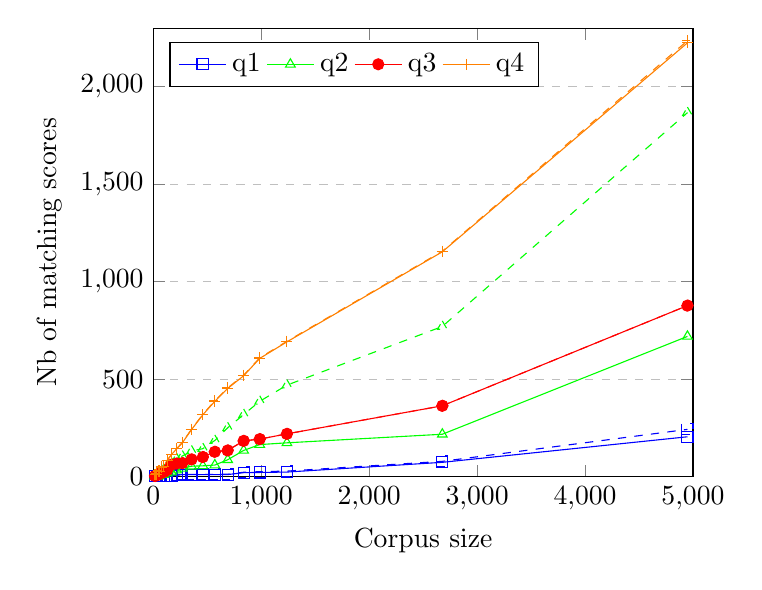
\begin{tikzpicture}[scale=1]
	\begin{axis}[
	xlabel={Corpus size},
	ylabel={Nb of matching scores},
	xmin=0, xmax=5000,
	ymin=0, ymax=2300,
	legend pos=north west,
	ymajorgrids=true,
	grid style=dashed,
	legend style={legend columns=4},
%    ybar,
%    bar width=0.1cm,
%symbolic x coords={16, 33, 53, 75, 97, 128, 169, 216, 269, 354, 459, 570, 689, 837, 986, 1238, 2678, 4949	},
%x tick label style={rotate=90,anchor=east},
%xtick=data,	%ymode=log,
	%xmode=log,
	]
	
    \addplot[
        color=blue,
        mark=square,
        ]
        coordinates {
(16,4)
(33,4)
(53,4)
(75,4)
(97,4)
(128,4)
(169,4)
(216,7)
(269,10)
(354,10)
(459,10)
(570,10)
(689,10)
(837,20)
(986,21)
(1238,23)
(2678,73)
(4949,204)
 };

    \addplot[
color=blue,
        mark=square,
dashed
]
coordinates {
(16,4)
(33,4)
(53,4)
(75,4)
(97,4)
(128,4)
(169,4)
(216,7)
(269,11)
(354,11)
(459,11)
(570,11)
(689,12)
(837,22)
(986,25)
(1238,28)
(2678,78)
(4949,242)
};
\addplot[
        color=green,
        mark=triangle,
        ]
        coordinates {
(16,0)
(33,1)
(53,2)
(75,10)
(97,10)
(128,18)
(169,23)
(216,33)
(269,42)
(354,53)
(459,55)
(570,59)
(689,86)
(837,134)
(986,164)
(1238,173)
(2678,217)
(4949,719)        };

\addplot[
color=green,
        mark=triangle,
dashed
]
coordinates {
(16,5)
(33,8)
(53,21)
(75,33)
(97,34)
(128,50)
(169,67)
(216,91)
(269,105)
(354,131)
(459,143)
(570,185)
(689,250)
(837,318)
(986,386)
(1238,469)
(2678,770)
(4949,1867)
};

\addplot[
        color=red,
        mark=*,
        ]
        coordinates {
(16,3)
(33,6)
(53,13)
(75,22)
(97,23)
(128,33)
(169,61)
(216,67)
(269,69)
(354,88)
(459,100)
(570,127)
(689,134)
(837,183)
(986,192)
(1238,219)
(2678,363)
(4949,877)
        };

\addplot[
color=red,
        mark=*,
dashed
]
coordinates {
(16,3)
(33,6)
(53,13)
(75,22)
(97,23)
(128,33)
(169,61)
(216,67)
(269,69)
(354,88)
(459,100)
(570,127)
(689,134)
(837,183)
(986,192)
(1238,219)
(2678,363)
(4949,877)
};

\addplot[
        color=orange,
        mark=+,
        ]
        coordinates {
(16,11)
(33,12)
(53,28)
(75,49)
(97,52)
(128,82)
(169,113)
(216,142)
(269,173)
(354,241)
(459,317)
(570,386)
(689,452)
(837,517)
(986,606)
(1238,691)
(2678,1153)
(4949,2225)
        };

\addplot[
color=orange,
        mark=+,
dashed
]
coordinates {
(16,12)
(33,13)
(53,29)
(75,50)
(97,53)
(128,83)
(169,114)
(216,143)
(269,175)
(354,243)
(459,319)
(570,389)
(689,455)
(837,520)
(986,609)
(1238,694)
(2678,1156)
(4949,2236)
};

	
	\legend{q1, , q2, , q3, , q4, }
	\end{axis}
	\end{tikzpicture}
		\vspace*{-.75cm}
		\caption{\label{fig:matchingRatio} Nb of matching with and without synonyms}
\end{minipage}
\input{figs/executionTime.tex}
\end{figure*}

The integration of our approach in \elasticsearch/ needs to preprocess musical scores to normalize them, and to compute the ranking in the search engine on query-time.

The first step consists in a Python scripts that normalizes voices from scores (Alg.~\ref{alg:norm}), extracts \textit{n}-grams, and produce JSON documents sent to the \elasticsearch/ REST API. Documents also contain corpus and opus ids, syllables from lyrics voices which can be queried.% to get more relevant and complex queries.

%\remNT{Ce n'est peut être pas utile que je rajoute un document JSON stocké (ngram + voix) ?}

Second, to take into account synonyms in \elasticsearch/, the list of \textit{n}-gram synonyms needs to be set %to the REST API\footnote{\url{https://www.elastic.co/guide/en/elasticsearch/guide/current/using-synonyms.html}}
offline. We have generated the list of all combinations of third and sixth transformation for each possible \textit{n}-gram available in the repository.
This list is imported in \elasticsearch/ and then processed on-the-fly for each query.

The third step integrates the \texttt{ScoreSim} scoring module as a Java program in \elasticsearch/.
For this, a \textit{SearchScript} needs to be inherited in order to produce a plugin for \elasticsearch/.
This plugin takes queries' parameters and instantiates a scoring function which will process every matching scores.
The scoring function \texttt{ScoreSim} implements  Algorithms~\ref{alg:occurrences} %(finding block occurrences)
 and \ref{alg:ranking}.% (producing scores for ranking).

The query below integrates all features that are proposed in our approach: \textit{n}-gram 
search (\textit{melody.value}), synonyms analyzer (\textit{melodic\_transformation}), and 
the \texttt{ScoreSim} function (\textit{script\_score}). In the latter, the parameter 
``\textit{query}'' gives the list of pitches used in order to produce the score value from Algorithm~\ref{alg:ranking}.
The query params gives the sequence of the music items (octave, pitch and duration) that constitutes 
the pattern in order to provide distances and rank the result set.
%An excerpt is shown in Example~\ref{ex-query}.
%Note that we also store the id of each item, which is actually the id of the corresponding element in the XML encoding of the score. 
%\begin{Example}\label{ex-query}~

\vspace*{-.2cm}
\begin{tiny}
	\begin{minted}{json}
{"query":{ "function_score": {
    "query": { "match_phrase": { "melody.value": "mcbb",
                       "analyzer": "melodic_transformation"}},
    "functions": [{"script_score": {
      "script": {"source": "scorelib", "lang": "ScoreSim",
        "params": {"query":[
            {"s":"A", "o":4, "id":"m42", "a":0, "d":8.0},
            {"s":"E", "o":3, "id":"m43", "a":0, "d":4.0},
            {"s":"G", "o":3, "id":"m44", "a":0, "d":4.0},
            {"s":"B", "o":4, "id":"m45", "a":0, "d":6.0}]}}}}]}}} 
  \end{minted}
\end{tiny}
%\end{Example}

Figure~\ref{../figures/Elasticsearch-implem} shows the querying process with the following steps: \textbf{1)} transform the melodic pattern into the \elasticsearch/ DSL (Domain Specific Language), \textbf{2)} \elasticsearch/ gets all the matching score corresponding to the given \textit{n}-gram and eventually to their synonyms, \textbf{3)} instantiate the \texttt{ScoreSim} plugin and process every score, \textbf{4)} extract occurrences on each instance and then its score value, \textbf{5)} and finally, \elasticsearch/ sorts the whole result-set according to the produced scores and sends the result.

\subsection{Performance}

%Due to space restrictions, we limit the report of our performance evaluation to scalability aspects.

In order to study the impact of our approach on the computation time, 
we apply different queries on our corpora. The corpora size varies by cumulating  several 
corpus, representing up to  4,950  polyphonic scores. It is composed of the whole corpora available here\footnote{\neuma/ repertory: \url{http://neuma.huma-num.fr/home/}} composed of \textit{Franc\oe{}ur, M\'ethodes, Motet, Psautiers, Sequentia, Timbres}, etc.

\begin{table}[t]
	\footnotesize
	\begin{tabular}{p{2.8cm}|c|c|c|c}
		& q1 & q2 & q3 & q4\\
		\hline
		Querying pattern & \texttt{demc} & \texttt{mcmcmc} & \texttt{bmbb} & \texttt{bmbmc}\\
		\hline
		Nb of matching scores & 204 & 719 & 877 & 2,225\\
		\hline
		Nb with query expansion & 242 & 1867 & 877 & 2,236\\ \hline
	\end{tabular}
	\caption{\label{tab:queryPatterns}Query patterns}
\end{table}

To study the effect of the matching process, we have chosen four different queries to apply with various patterns, from infrequent to more frequent ones,
based on the popularity of the stored \textit{n}-grams. 
Table~\ref{tab:queryPatterns} gives for each query pattern the corresponding total number of matches in the corpora and the number after applying the query expansion (synonyms). We can see that query q2 is clearly expanded since \texttt{mcmcmc} has 7 synonyms and produces a large number of matches (2.5 times more). At the opposite, query q3 has no synonyms and do not enlarge its result-set.

Figure~\ref{fig:matchingRatio} shows the evolution of the number of matching scores wrt 
the corpus size. It gives both matching scores for normal (plain lines) and expanded queries (dashed lines). 
%Each query follows a specific ratio of matchings and is globally homogeneous all over the corpora. 
According to the synonyms, we can see that q1 and q4 provide few more matchings, while q2 witnesses a different behavior where the number of matchings grows proportionally with the number of synonyms.
%It will help to see how the query expansion impacts performances.


The execution time is plotted in Figure~\ref{fig:executionTime} for the 4 different queries.
It shows both normal pattern queries (plain lines) and expanded queries (dashed lines).
This allows to investigate both the robustness 
with respect to various results sizes, and issues related to false positives.

Each query is sub-linear in the result size. Query q4 is a frequent pattern
which returns 2,225 matching scores (45\% of the corpora). It is executed in 277 ms. The small number of synonyms has few impacts on the global processing time.
At the opposite, q1 is extremely efficient due to its selectivity. It produces  204 scores in 22 ms.
One interesting effect can be seen for query q2 where the number of matching synonyms leads to more computation time but it only 2.1 times more (for 2.5 times more matching scores).


% \begin{figure}[ht]
%   \centerline{
%     \includegraphics[width=.45\textwidth]{figs/executionTime.png}}
%   \caption{\label{fig:executionTime} Execution time with respect to corpus size}
% \end{figure}
 
%\input{figs/executionTimeSynonyms.tex}

%\begin{figure}[h]
	\begin{tikzpicture}[scale=1]
	\begin{axis}[
	xlabel={Corpus size},
	ylabel={Time per score (ms)},
	xmin=0, xmax=5000,
	% ymin=0, ymax=30,
	legend pos=north east,
	ymajorgrids=true,
	grid style=dashed,
	ymode=log,
	%xmode=log,
	]
	
	    \addplot[
        color=blue,
        mark=square,
        samples=100
        ]
        coordinates {
(0,9)
(16,2.6)
(33,2.4)
(53,2.4)
(75,2.4)
(97,2.4)
(128,2.4)
(169,2.4)
(216,1.5)
(269,1.08333333333333)
(354,1.08333333333333)
(459,1.16666666666667)
(570,1.16666666666667)
(689,1.07692307692308)
(837,0.695652173913043)
(986,0.730769230769231)
(1238,0.758620689655172)
(2678,0.316455696202532)
(4949,0.135802469135802)
 };

	\input{figs/executionPerScoreSynonyms-plot2}
	\input{figs/executionPerScoreSynonyms-plot3}
	\addplot[
        color=orange,
        mark=+,
        ]
        coordinates {
(0,4)
(16,1.15384615384615)
(33,1.42857142857143)
(53,0.866666666666667)
(75,0.647058823529412)
(97,0.722222222222222)
(128,0.547619047619048)
(169,0.469565217391304)
(216,0.423611111111111)
(269,0.392045454545455)
(354,0.364754098360656)
(459,0.33125)
(570,0.312820512820513)
(689,0.300438596491228)
(837,0.312859884836852)
(986,0.30327868852459)
(1238,0.317985611510791)
(2678,0.210025929127053)
(4949,0.13455520786768)
        };

	
	\legend{q1, q2, q3, q4}
	\end{axis}
	\end{tikzpicture}
	\caption{\label{fig:timeVSsizeSynonyms} Execution time per score with respect to corpus size with query expansion}
\end{figure}


%
%
%To study the time spent per score, Figure~\ref{fig:timeVSsize} gives in log scale the average time to process each score with respect to the corpus size.
%We can see that an initial cost is visible at the beginning of the curves, this constant penalty is associated to the initialization of the \texttt{ScoreSim} user-defined similarity function and levels up the average computation time.
%For small corpus, computing a score depends mostly on the number of occurrences found in voices (q1) which can vary from one corpus to another.
%Fortunately this effect is smoothed for bigger corpus even for frequent patterns or expanded queries, the ranking function takes less than 0.12ms to process each score.
% 
% \pgfplotsset{width=.98\linewidth, height=5cm}
\begin{figure}[h]
	\begin{tikzpicture}[scale=1]
	\begin{axis}[
	xlabel={Corpus size},
	ylabel={Time per score (ms)},
	xmin=0, xmax=5000,
	ymin=0.09, ymax=10,
	legend pos=north east,
	ymajorgrids=true,
	grid style=dashed,
	ymode=log,
	%xmode=log,
	]
	
	\input{figs/executionPerScore-plot1}
	\input{figs/executionPerScore-plot2}
	\input{figs/executionPerScore-plot3}
	\addplot[
        color=orange,
        mark=+,
        ]
        coordinates {
(0,2)
(16,0.666666666666667)
(33,0.769230769230769)
(53,0.517241379310345)
(75,0.46)
(97,0.528301886792453)
(128,0.421686746987952)
(169,0.394736842105263)
(216,0.363636363636364)
(269,0.344827586206897)
(354,0.330578512396694)
(459,0.311320754716981)
(570,0.302325581395349)
(689,0.293598233995585)
(837,0.295366795366795)
(986,0.2833607907743)
(1238,0.297687861271676)
(2678,0.197573656845754)
(4949,0.124887690925427)
        };

\addplot[
color=orange,
dashed,
mark=+,
]
coordinates {
	(0,4)
	(16,1.15384615384615)
	(33,1.42857142857143)
	(53,0.866666666666667)
	(75,0.647058823529412)
	(97,0.722222222222222)
	(128,0.547619047619048)
	(169,0.469565217391304)
	(216,0.423611111111111)
	(269,0.392045454545455)
	(354,0.364754098360656)
	(459,0.33125)
	(570,0.312820512820513)
	(689,0.300438596491228)
	(837,0.312859884836852)
	(986,0.30327868852459)
	(1238,0.317985611510791)
	(2678,0.210025929127053)
	(4949,0.13455520786768)
};

	
	\legend{q1, , q2, , q3, , q4, }
	\end{axis}
	\end{tikzpicture}
	\caption{\label{fig:timeVSsize} Execution time per score with respect to corpus size  with and without query expansion}
\end{figure}

Those experiments show that the ranking function takes less than 0.12 ms to process each score on a single \elasticsearch/ node (server). The corpus can be spread on several nodes in order to scale it up horizontally.
 
 
\section{Related work}\label{sec:rw}

Our approach combines similarity searches based on textual music encoding, 
scalable search, and rhythm-based ranking.
The novelty of this approach is their association in a consistent setting.
The rather trivial implementation makes, in our opinion, our solution quite attractive. 

%\subsection{Related Work}
% Similarity
Music similarity has been an active MIR research topic over the last decades~\cite{Casey2008}. The general
goal is to evaluate the likeness of two musical sequences. %, in a way that matches as much as possible the human listener perception.
A major problem raised by this definition
is that similarity judgments are highly dependent on both the content being compared and
on the user taste, culture, and experience~\cite{JDE07,ERP17}. 
%This encourages  a proliferation of methods, often originated from different fields, and makes difficult their comparison.
%The following is a brief overview that positions our approach. 
A recent survey~\cite{Velardo2016}
summarizes the recent trends observed in the SMS track of the MIREX competition.

A similarity method is characterized by the choice of musical parameters. Pitches and durations  
are generally considered as expressive enough. 
Using sequences to represent both parameters is primarily motivated by 
our objective to integrate our methods in a standard search engine, and to benefit from an index structure.
%This eliminates more complex representations where the price to pay is a less expressive matching semantic.
Some important parameters,
e.g., metric accent, structure or harmonic 
are ignored because they often lead to tree-based encodings that are hardly indexable. Geometric approaches,
such as~\cite{TGVWO03},
are also less suitable in this indexing perspective. Multidimensional structures are complex, 
and their  performances are known to
fall down as the dimension increases~\cite{Samet2006}, and not yet integrated to off-the-shell search engines.

% Textual encoding
Textual encoding of symbolic music representation is an attractive idea
in order to use text algorithms. The \textit{HumDrum} toolkit~\cite{Knopke08}
relies on a specialized text format and adapts Unix file inspection tools for music analysis. 
Exact and approximate
string matching algorithms for melody matching have been used in \textit{ThemeFinder}~\cite{Kornstaedt98,Stuart_search-effectivenessmeasures} or \textit{Musipedia}~\cite{PLT01}.
Many algorithms for efficient
computation of similarity matching through exhaustive searches
have been proposed~\cite{CCF04,CCF05,CI04,CCIMS05}. 
Specialized rhythm similarity functions are proposed and compared in~\cite{Toussaint04}.

Text-based approaches are simple solutions, with two important limitations. First, %these methods are designed for text and are not well adapted to the specificities of music representation. 
combining pitches and rhythm in a single character string for instance is not easy, 
and small music variants may result in important syntactic differences.  %Since, in addition, we usually search for a match between a query pattern and any subsequence of a voice, encoding, it is unclear which substrings have to be chosen before applying the approximate matching operation. 
% Scalability
Second, these methods
do not scale since the whole database has to be inspected for each query.
%Text matching algorithms are not always easily supported by an index. 
%In the specific context of the edit distance, 
Several indexing methods have been suggested for the edit distance~\cite{Navarro00,ConstantinMFR11}.
The \textit{Dynamic Time Warping} distance is another popular method, for which sophisticated indexing structures
have been proposed~\cite{KR05,Klaus18}. None of them is available beyond research prototypes.

The easiest way to benefit
from an inverted index is to split musical sequences in $n$-grams. This has been
experimented in several earlier proposals~\cite{Downie99,NO04,DR04,CJ06}. Each $n$-gram plays the role
of a ``token'' and search methods apply. %Keywords search will retrieve a sequence even though a subset of the $n$-gram match those of the patterns.
%This is somewhat similar to a similarity search.
%Phrase search, on the other hand, corresponds to an exact search of the indexed sequence. The flexibility lies
%in the pre-processing transformation applied to both the stored sequence and the query pattern.

Ranking is an essential part of an information retrieval system. %Any query with a few keywords retrieves from the Web millions of documents. 
%The quality of the result is mostly estimated by the ability of the search engine to top-rank the most relevant ones.
We believe that our proposal, which combines \textbf{1)}~a pre-processing normalization step,
 \textbf{2)} a melodic profile search and \textbf{3)} a rhythmic profile ranking, completes earlier
attempts to adapt text-based retrieval to music retrieval, and results in a complete workflow
which achieves a satisfying trade-off between the filtering impact, the ranking relevancy and
the overall efficiency.

% Ranking



\section{Conclusion}\label{sec:conclusion}

We described in this paper a practical approach to the problem of indexing
pattern-based searches in a large score library. Our solution fulfills three major 
requirements for an information retrieval system: (i) it supports search with 
a significant part of flexibility, (ii) it proposes a ranking method consistent with
the matching definition, and (iii) it brings scalability thanks to its
compatibility  with the features of state-of-the-art search engines.  We fully 
implemented our solution, including the internal ranking function for \elasticsearch/,
and we will be pleased to supply our software components to any interested institution
that wishes to propose a content-based search mechanism.% to its users.
%We are currently working on an open-source release of our packages on GitHub.
 
%The proposal presented in this paper is by no way a final achievement. Several extensions can be envisaged. Let us mention the ones that seem most promising at the time of writing.

\noindent
\textbf{Score analyzers extension.} Alg.~\ref{alg:norm} with the normalization of voices can be extended with
ad hoc music \emph{analyzers}: management of grace notes, the simplification of melodic profiles, treatment of repeated notes, or cross-voice melodies, to
name a few.
% propose numerous methods of text processing that can be combined in order to form a dedicated \emph{analyzer}. We can do the same thing for music indexing, letting the  depending on her needs.

\noindent 
\textbf{Acknowledgments.} This work is funded by the French ANR project
\munir/ %(\url{http://www.neuma.fr}).


%\bibliography{ISMIRtemplate}
\bibliography{../biblio}



%\begin{figure*}[ht]
% \centerline{
% \includegraphics[width=\textwidth]{../figures/screenshot-search}}
% \caption{\label{screenshot-search} The search interface of \neuma/, highlighting matching occurrences}
%\end{figure*}

\end{document}
